\documentclass[a4paper, 12pt]{article}
\usepackage[utf8]{inputenc}
\usepackage{geometry}
\usepackage{polski}
\usepackage{graphicx}
\usepackage{float}
\usepackage{etoolbox,refcount}
\usepackage{multicol}

\newgeometry{left=2cm, right=2cm, bottom=1.5cm, top=1.5cm}

\begin{document}
	\begin{figure}[H]
		\centering
		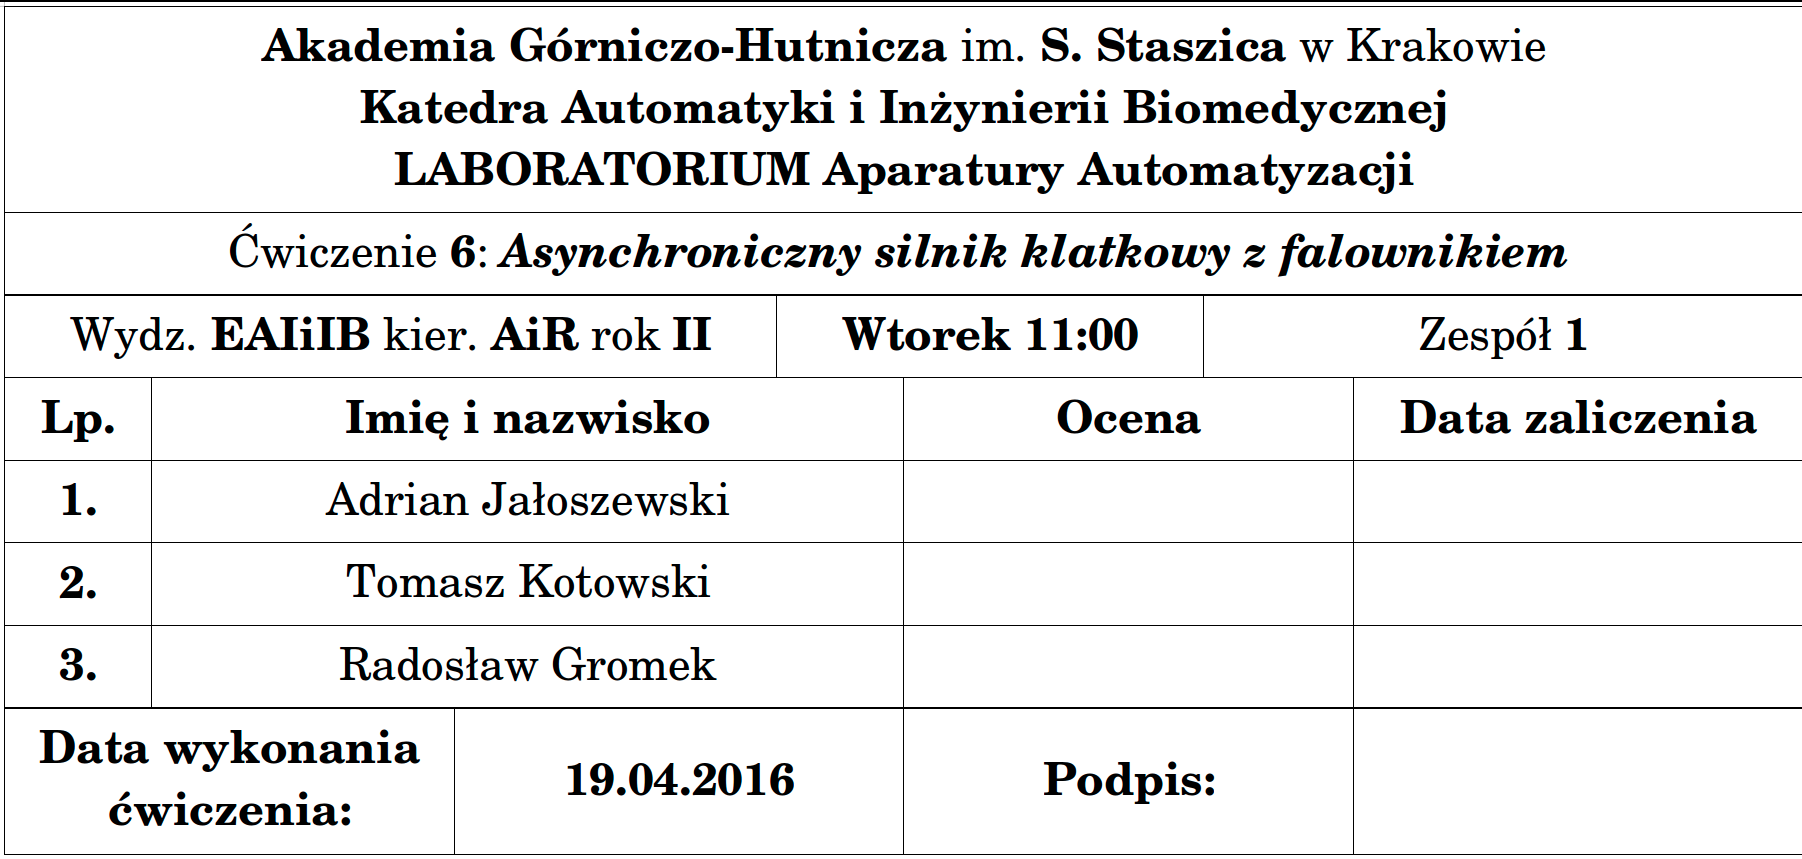
\includegraphics[height=6cm, width=\textwidth]{./img/cudo.png}
	\end{figure}
	\section{Cel ćwiczenia}
		Celem ćwiczenia jest zapoznanie się z konfiguracją i uruchomieniem silnika elektrycznego\linebreak z falownikiem przy pomocy oprogramowania SINAMICS 4.4 STARTER.
	\section{Schemat stanowiska}
		\begin{figure}[H]
			\centering
			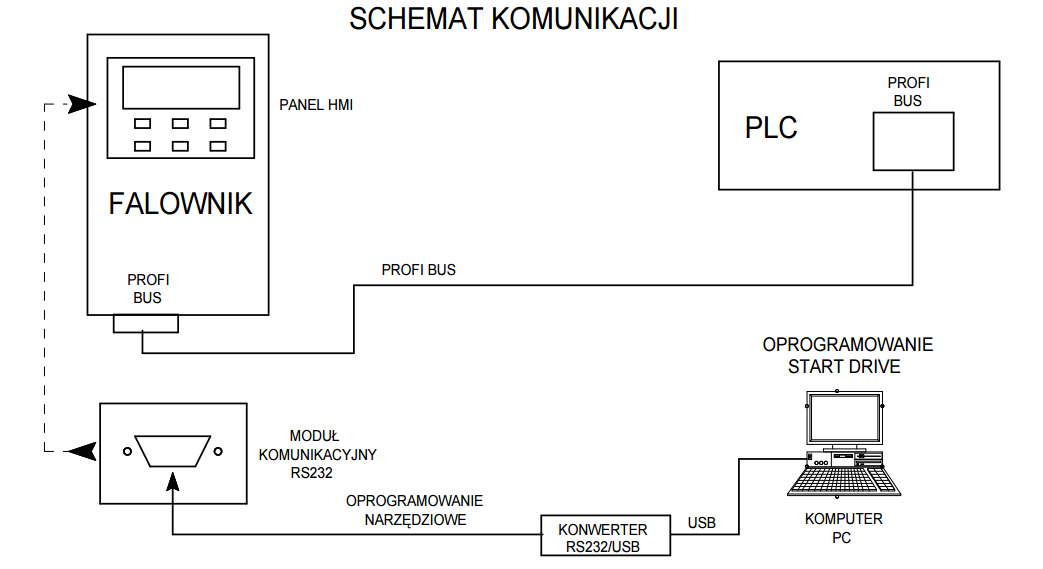
\includegraphics[width=\textwidth]{./img/stanowisko.png}
		\end{figure}
		Stanowisko składa się z komputera klasy PC z konwerterem USB-RS232 oraz oprogramowaniem konfiguracyjnym, falownika, silnika indukcyjnego, zespołu przełączników z potencjometrem do sterowania ręcznego oraz ręcznego laserowego czujnika prędkości obrotowej.
	\section{Przebieg ćwiczenia}
		Ćwiczenie rozpoczęliśmy od uruchomienia oprogramowania służącego do sterowania silnikiem przy pomocy falownika. Następnie skonfigurowaliśmy połączenie pomiędzy środowiskiem konfiguracyjnym i falownikiem korzystając z Wizarda. Następnie ustaliliśmy parametry układu oraz załadowaliśmy obiekt do targetu. Po dokonaniu tego zdefiniowaliśmy tabelę do monitorowania zmiennych, w której uwzględniliśmy częstotliwość, prędkość obrotową, napięcie na wejściu analogowym oraz napięcie stałe na wejściu falownika.
		\newline 
		\newline
		Następnie otworzyliśmy panel sterujący, odblokowując możliwość uruchomienia napędu i zaznaczyliśmy możliwość zadania częstotliwości bazowej. Następnie dla sprawdzenia działania napędu sprawdziliśmy cztery ustawienia - odpowiednio -50, -25, 25 oraz 50 Hz. Zgodnie z przewidywaniami dla częstotliwości ujemnych silnik kręcił się przeciwnie niż robił to dla częstotliwości dodatnich, a dla częstotliwości o większym module kręcił się szybciej niż dla częstotliwości\linebreak o mniejszej wartości bezwzględnej.
		\subsection{Prędkość od zadanej częstotliwości, $\frac{V}{f} = const$}
			W pierwszej serii pomiarów mieliśmy zbadać charakterystykę statyczną dla silnika zmieniając częstotliwość w zakresie od 5 do 50 Hz co 5 Hz. Pomiar miał być dokonany poprzez odczyt\linebreak z czujnika laserowego trzymanego w ręce oraz z panelu.
			\begin{center}
				\begin{tabular}{|c|c|c|c|}
					\hline f[Hz] & Czujnik[rpm] & Panel[rpm] & Różnica \\ 
					\hline 5 & 148,8 & 149,963 & 1,163 \\ 
					\hline 10 & 298,3 & 299,926 & 1,626 \\ 
					\hline 15 & 447,8 & 449,981 & 2,181 \\ 
					\hline 20 & 597,4 & 599,945 & 2,545 \\ 
					\hline 25 & 747,3 & 750 & 2,7\\ 
					\hline 30 & 897 & 899,963 & 2,963 \\ 
					\hline 35 & 1046 & 1049,927 & 3,927 \\ 
					\hline 40 & 1196 & 1199,982 & 3,982\\ 
					\hline 45 & 1346 & 1349,945 & 3,945\\ 
					\hline 50 & 1496 & 1500 & 4\\ 
					\hline 
				\end{tabular}
			\end{center}
			Poniższy wykres przedstawia tę zależność dla pomiarów odczytanych z panelu:
			\begin{figure}[H]
				\centering
				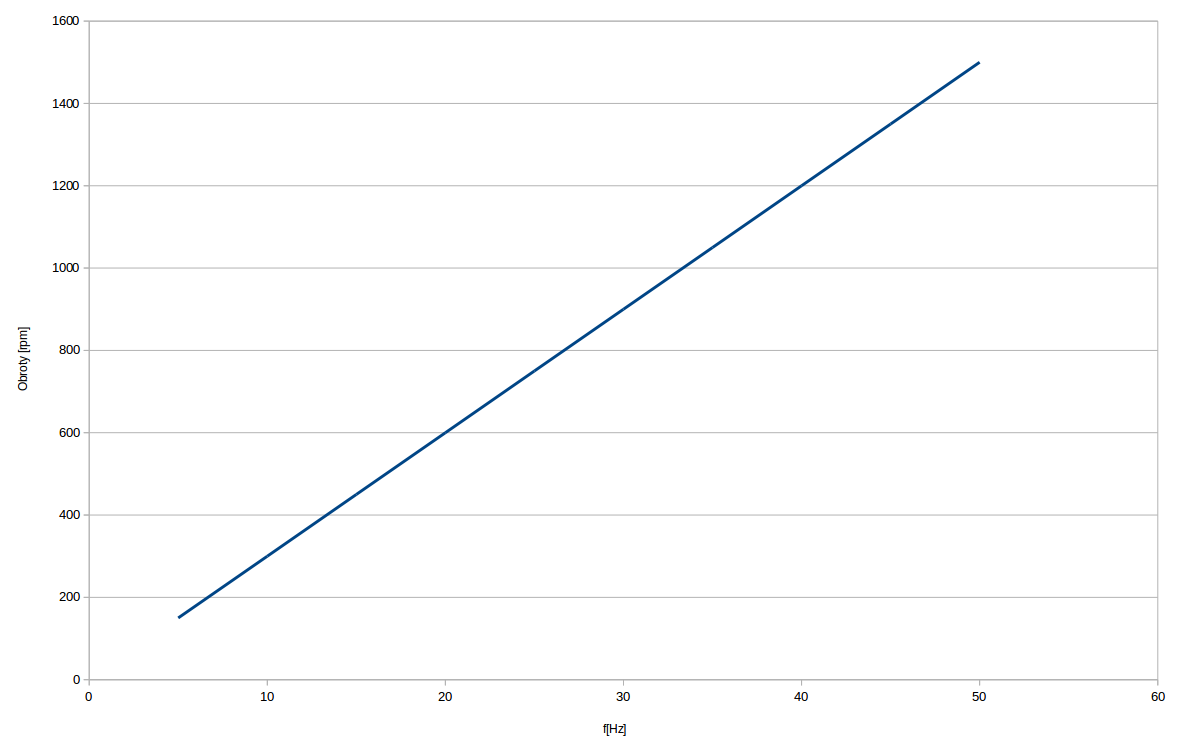
\includegraphics[width=\textwidth]{./img/pierwsze.png}
			\end{figure}
			\noindent Różnice pomiędzy odczytem z panelu oraz z czujnika biorą się stąd, że mamy do czynienia\linebreak z wartością chwilową w przypadku czujnika, a nie z uśrednieniem wielu próbek tak jak w odczycie z panelu. Dodatkowo całość jest zaburzona lekkimi drganiami ręki osoby dokonującej pomiarów oraz możliwością dokonania pomiarów pod niewielkim kątem.
		\subsection{Charakterystyka liniowa}
			Do wykonania tej charakterystyki musieliśmy najpierw wyjść z panelu sterującego i uruchomić falownik przełącznikiem start/stop.
			\begin{center}
				\begin{tabular}{|c|c|c|c|}
					\hline $U_{adc}$[V] & Czujnik[rpm] & Panel[rpm] & Napięcie[V] \\ 
					\hline 0 & 148,8 & 150 & 34,114\\ 
					\hline 1,036 & 302,2 & 303,9 & 54,631\\ 
					\hline 1,994 & 447,7 & 449,1 & 74,78\\ 
					\hline 2,991 & 596 & 598,608 & 96,219\\ 
					\hline 4,027 & 751 & 755,146 & 119,285\\ 
					\hline 5,024 & 900 & 903,662 & 141,161 \\ 
					\hline 6,031 & 1049 & 1053,475 & 163,605 \\ 
					\hline 7,028 & 1200 & 1203,815 & 186,118\\ 
					\hline 7,986 & 1346 & 1349,03  & 207,591\\ 
					\hline 9,012 & 1496 & 1500 & 228,031\\ 
					\hline 10 & 1496 & 1500 & 226,765\\ 
					\hline 
				\end{tabular} 
			\end{center}
			Poniższy wykres przedstawia tę zależność dla pomiarów odczytanych z panelu:
			\begin{figure}[H]
				\centering
				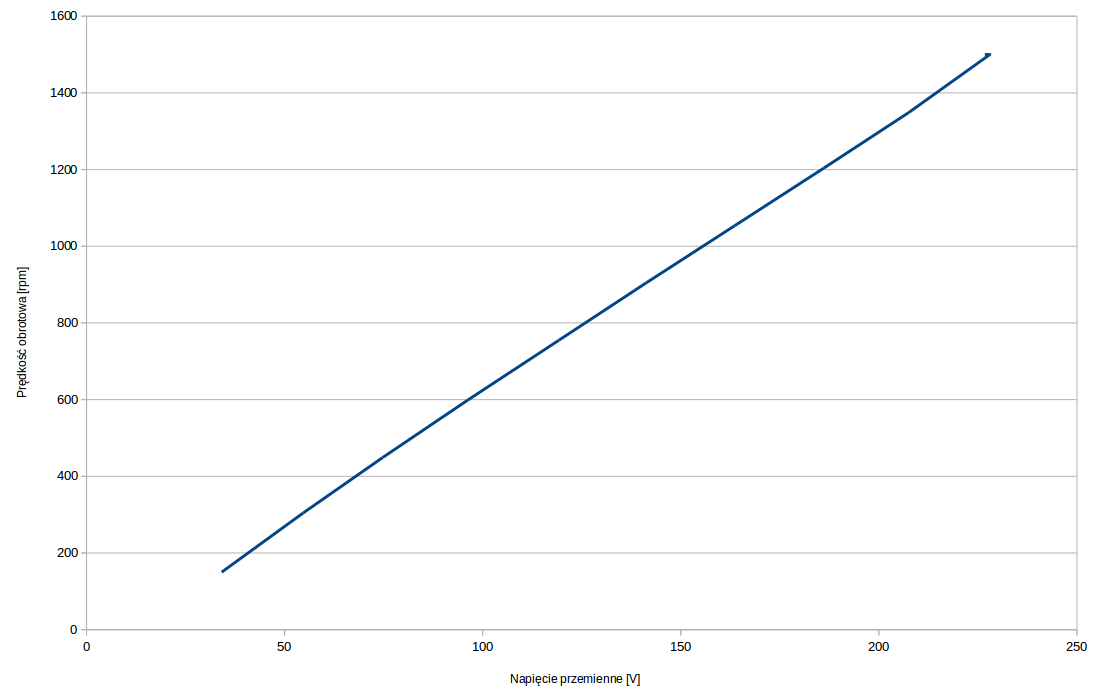
\includegraphics[width=\textwidth]{./img/drugie.png}
			\end{figure}
		\subsection{Charakterystyka paraboliczna}
			Wykonanie tej części ćwiczenia musieliśmy rozpocząć od ponownego skonfigurowania falownika, tak aby dawał nam na wyjściu napięcie proporcjonalne do kwadratu częstotliwości $\frac{V}{f^2} = const$. Następnie wgraliśmy nową konfigurację, pozostawiając pozostałe parametry przy tej samej wartości.
			\begin{center}
				\begin{tabular}{|c|c|c|c|}
					\hline $U_{adc}$[V] & Czujnik[rpm] & Panel[rpm] & Napięcie[V]  \\ 
					\hline 0 	& 148,5	& 150 		& 18,89  \\ 
					\hline 1,026& 304,2 & 306,21 	& 29,98 \\ 
					\hline 2,04 & 453 	& 454,58 	& 45,28 \\ 
					\hline 3,02 & 601 	& 603,54 	& 64,34 \\ 
					\hline 4,027& 751,5 & 752,83 	& 86,72 \\ 
					\hline 4,985& 895,5 & 898,32 	& 110,79\\ 
					\hline 6,031& 1051 	& 1054,32 	& 138,54\\ 
					\hline 7,038& 1200 	& 1204,23 	& 167,41\\ 
					\hline 8,01 & 1350 	& 1353,73 	& 198,25\\ 
					\hline 9,012& 1496 	& 1500 		& 227,71\\ 
					\hline 10 	& 1496 	& 1500 		& 228,031\\ 
					\hline 
				\end{tabular} 
			\end{center}
			Poniższy wykres przedstawia tę zależność dla pomiarów odczytanych z panelu:
			\begin{figure}[H]
				\centering
				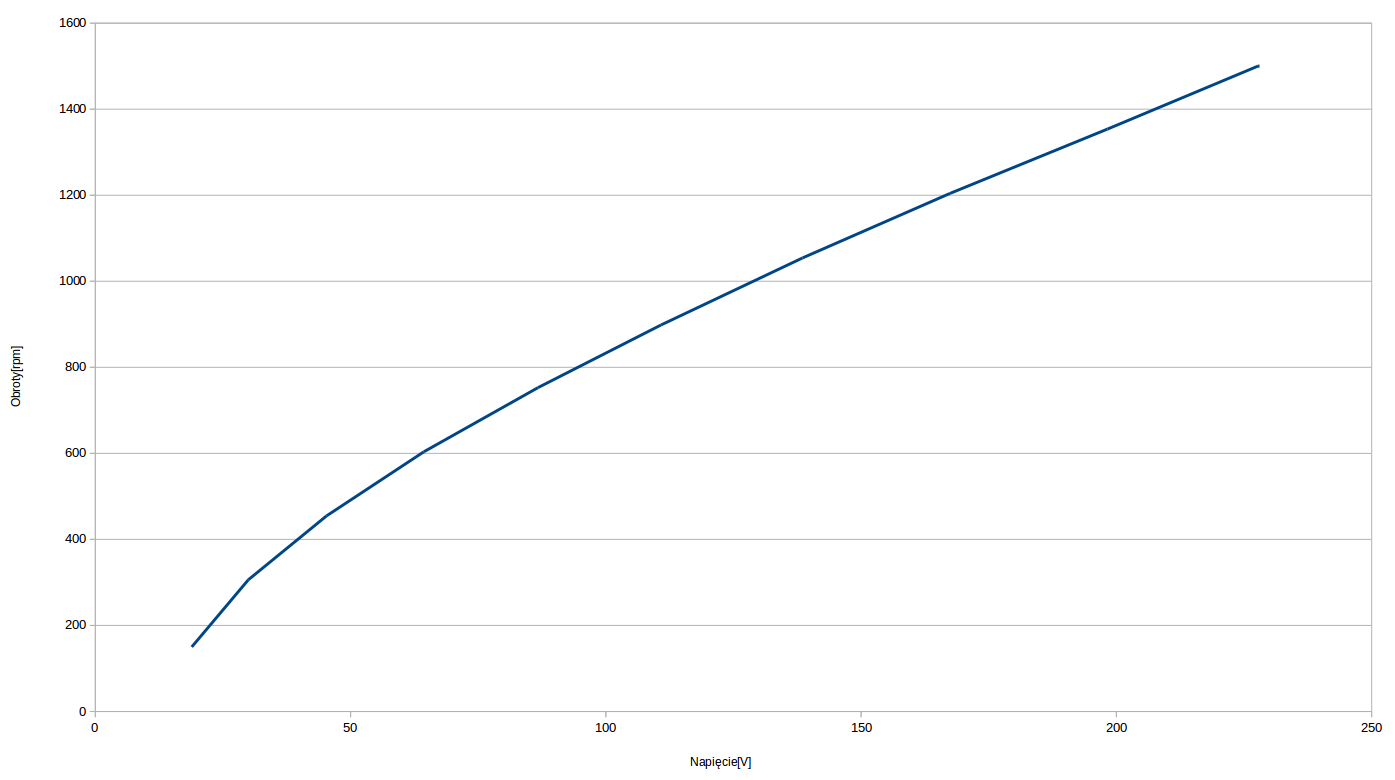
\includegraphics[width=\textwidth]{./img/trzecie.png}
			\end{figure}
	\section{Wnioski}
		Ćwiczenie te pozwoliło nam na zapoznanie się z metodami sterowania silnikami indukcyjnymi oraz pozwoliło nam poznać ich zachowania dla różnych sterowań falownikiem - jak mamy napięcie proporcjonalne do kwadratu częstotliwości oraz jak mamy napięcie proporcjonalne do częstotliwości.
		\newline
		\newline
		Zdecydowanie bardziej stabilne wyniki z panelu pokazały nam wygodę korzystania z tego typu narzędzi. Pomiary dokonywane przy pomocy miernika ręcznego szwankowały zdecydowanie bardziej oraz były trudniejsze w odczycie, gdyż musieliśmy trzymać miernik obrócony, aby otrzymać jak najdokładniejsze wyniki.
		\newline 
		\newline
		Mieliśmy w trakcie tych zajęć również możliwość zweryfikowania naszej wiedzy z zajęć z silników elektrycznych, gdyż nie mieliśmy tam okazji dokonania pomiarów dla charakterystyki parabolicznej.
		\newline
		\newline
		Zobaczyliśmy również jak szybko silnik klatkowy reaguje na zmiany zadanego sterowania. Na podstawie tych obserwacji stwierdziliśmy, że jest to czas zdecydowanie zbyt długi do wielu aplikacji wymagających precyzyjnej i szybkiej zmiany prędkości obrotowej silnika. Jednak dla wielu zastosowań jest to wystarczająco mały przedział czasu.
		\newline 
		\newline
		Szczególnie pouczająca była obserwacja czasu reakcji silnika pomiędzy dwoma skrajnymi ustawieniami częstotliwości zasilania. Zobaczyliśmy w ten sposób czas jaki musiał upłynąć zanim układ osiągnął stan ustalony.
\end{document}
